\begin{frame}
    \frametitle{Real-Time Inference and Prediction}
    \begin{itemize}
        \item Now we have a fast algorithm for applying \(\mathbf{F}\) and \(\mathbf{F}^*\) to vectors. How can we use that to enable real-time inference?
        \item Split inversion into \textbf{Offline} and \textbf{Online} phases:
        \begin{itemize}
            \item \textbf{Phase 1} (Offline): Construct p2o map from adjoint PDE solves
            \item \textbf{Phase 2} (Offline): Compute compact representation of \(\Gamma_{\!\text{post}}\)
            \item \textbf{Phase 3} (Online): Compute MAP point and QoI in real time
        \end{itemize}
        \item Offline/Online decomposition allows us to \emph{exactly\footnote{Exact up to discretization errors}} solve the inference and prediction problems in \(\mathcal{O}(\text{seconds})\) using the high-fidelity model.
        \begin{itemize}
            \item \textbf{No surrogates or reduced-order models necessary}
        \end{itemize}
    \end{itemize}
\end{frame}

\begin{frame}
    \frametitle{Phase 1: Constructing the p2o Map}
    \begin{itemize}
        \item Requires \(N_d\) adjoint PDE solves; solution vectors are of size \(N_mN_t\)
        \item PDE solution vectors define block lower-triangular Toeplitz matrix
    \end{itemize}
    \begin{figure}
        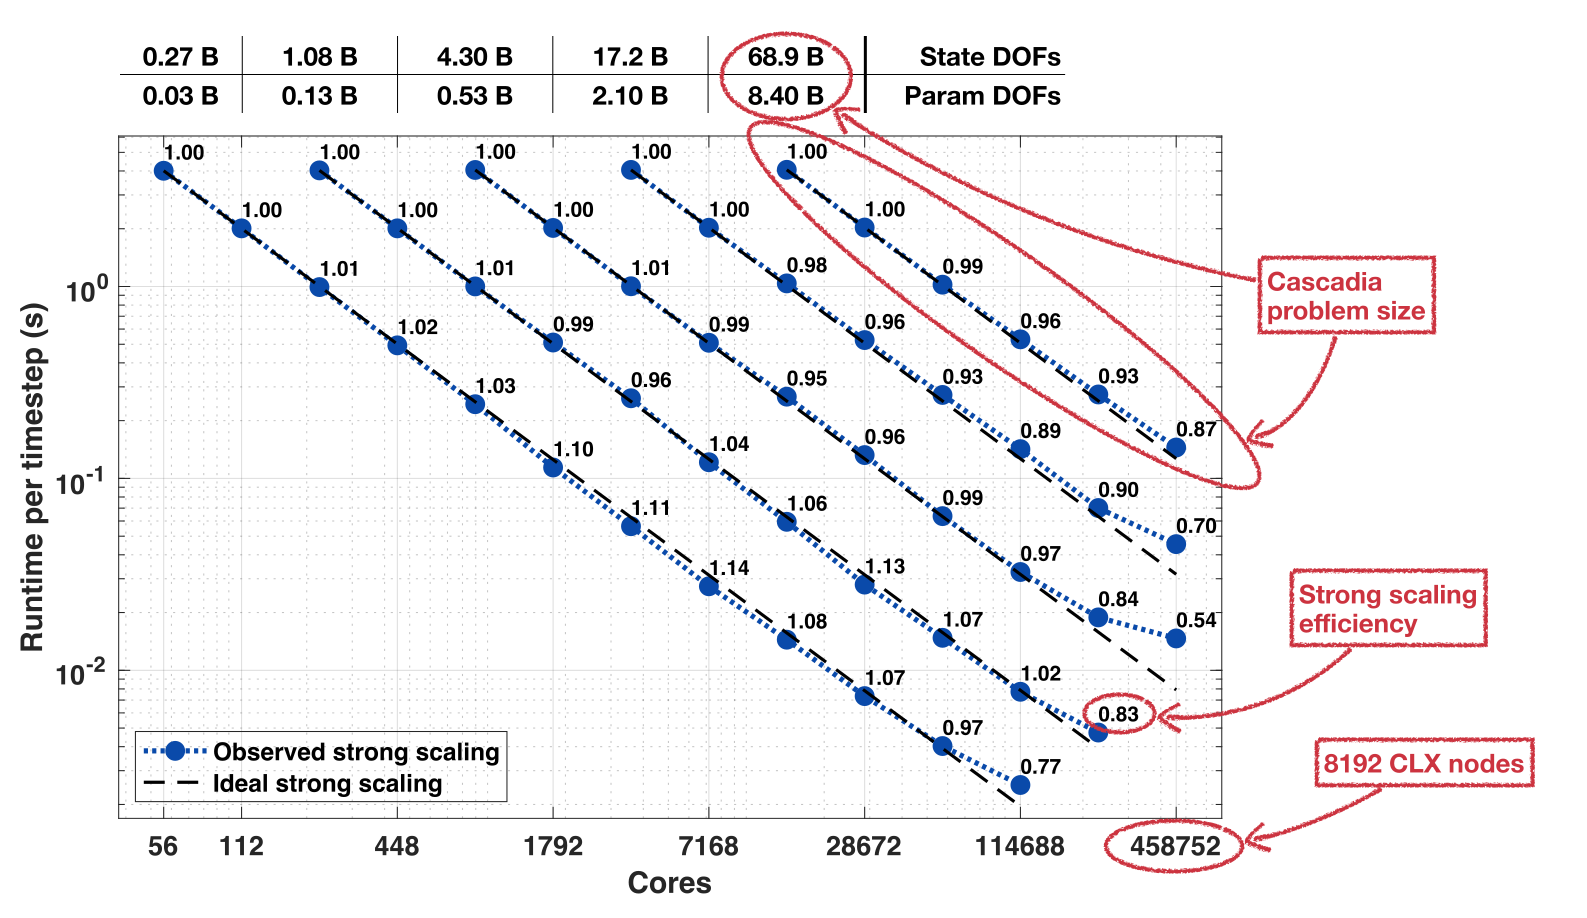
\includegraphics[width=\textwidth]{JMM/images/pde/Strong_Scaling.svg}
        \caption{Implemented by Stefan Henneking with MFEM}
    \end{figure}
\end{frame}
